% =====================================================================
%  Graduation Thesis
%  School of Engineering, Tohoku University
%  Department of Mechanical and Aerospace Engineering (IMAC)
%
%  Formatted to the departmental submission specification:
%    - A4, portrait, horizontal writing, two-sided, left-side binding
%    - Margins: top 20 mm, bottom 25 mm, binding (inner) 25 mm,
%               fore-edge (outer) 25 mm
%    - Page number centred in the bottom margin
%    - Figures placed inline in the body text
%    - No CV / curriculum vitae section
%
%  Build:  latexmk -pdf graduation_thesis.tex
%     or:  pdflatex -> biber -> pdflatex -> pdflatex
%  The separate spine sheet for binding is in spine.tex.
% =====================================================================

\documentclass[12pt, a4paper, twoside, openright]{report}

% --------------------------- Encoding & fonts ------------------------
\usepackage[utf8]{inputenc}
\usepackage[T1]{fontenc}
\usepackage{amsmath, amssymb}       % must precede newtxmath (\Bbbk clash)
\usepackage{newtxtext, newtxmath}   % Times New Roman-compatible text + math
\usepackage{microtype}

% --------------------------- Core packages ---------------------------
\usepackage{graphicx}
\usepackage{booktabs}
\usepackage{multirow}
\usepackage{siunitx}
\usepackage{float}
\usepackage{enumitem}
\usepackage{caption}
\usepackage{subcaption}
\usepackage{setspace}
\usepackage{fancyhdr}
\usepackage{emptypage}              % suppress headers/footers on blank versos
\usepackage[hidelinks]{hyperref}
% Citation style: IEEE numeric, i.e. bracketed [1] in the text, with the
% reference list ordered by first citation. This is the convention used across
% mechanical and aerospace engineering, and the department does not mandate an
% alternative. To switch to APA author-date instead, install biblatex-apa and
% replace the line below with:
%     \usepackage{csquotes}
%     \usepackage[backend=biber, style=apa]{biblatex}
% No other change is needed; the \cite commands in the body are style-agnostic.
\usepackage[backend=biber, style=ieee, sorting=none]{biblatex}

\graphicspath{{figures/}{figures/photos/}{../analysis/results/}}
\addbibresource{references.bib}

% Permit line breaks inside URLs/DOIs in the bibliography
\setcounter{biburllcpenalty}{7000}
\setcounter{biburlucpenalty}{8000}

% --------------------------- Page geometry ---------------------------
% Departmental spec: top 20 mm, bottom 25 mm, binding 25 mm, fore-edge 25 mm.
% `bindingoffset` is 0 because the binding allowance is already the full
% 25 mm inner margin required by the spec.
\usepackage[
    a4paper,
    top=20mm,
    bottom=25mm,
    inner=25mm,
    outer=25mm,
    footskip=12mm,      % keeps the page number inside the 25 mm bottom margin
    headsep=6mm
]{geometry}

\onehalfspacing

% Give TeX some slack on lines containing unbreakable \texttt{} file paths
\emergencystretch=3em

% --------------------- Headers and footers ---------------------------
% Page number centred in the bottom margin on every page, per the spec.
\pagestyle{fancy}
\fancyhf{}
\fancyfoot[C]{\thepage}
\renewcommand{\headrulewidth}{0pt}
\renewcommand{\footrulewidth}{0pt}

\fancypagestyle{plain}{%          % chapter-opening pages
    \fancyhf{}%
    \fancyfoot[C]{\thepage}%
    \renewcommand{\headrulewidth}{0pt}%
}

% --------------------------- Captions --------------------------------
\captionsetup{font=small, labelfont=bf, width=0.9\textwidth}
\captionsetup[sub]{font=small, labelfont=bf}

% --------------------------- Convenience -----------------------------
\newcommand{\thesistitle}{Tactile-Feedback Teleoperation: Grip Force and Grasping Performance Across Haptic Actuator Types for Fragile and Deformable Objects}
\newcommand{\authorname}{Adriel, Santoso, Imaran}
\newcommand{\studentid}{C2TB1701}          % TODO: insert actual student ID
\newcommand{\labname}{Hashimoto Laboratory}
\newcommand{\supervisorname}{Prof.\ Koichi Hashimoto}
\newcommand{\graduationdate}{September, 2026}

% Marks passages that are still placeholders in this draft.
\newcommand{\todo}[1]{\textit{[TODO: #1]}}

\begin{document}

% =====================================================================
%  COVER PAGE  (per the departmental cover sample)
% =====================================================================
\begin{titlepage}
    \centering
    \thispagestyle{empty}
    \singlespacing

    \vspace*{25mm}

    {\fontsize{18}{22}\selectfont Graduation Thesis\par}
    \vspace{6mm}
    {\fontsize{18}{22}\selectfont School of Engineering, Tohoku University\par}

    \vspace{40mm}

    {\fontsize{20}{26}\selectfont\bfseries \thesistitle \par}

    \vspace{40mm}

    {\fontsize{18}{22}\selectfont Department of Mechanical and Aerospace Engineering\par}
    \vspace{4mm}
    {\fontsize{18}{22}\selectfont \labname\par}

    \vspace{20mm}

    {\fontsize{18}{22}\selectfont \studentid\quad \authorname\par}

    \vfill

    {\fontsize{18}{22}\selectfont (\graduationdate)\par}

    \vspace*{20mm}
\end{titlepage}

\cleardoublepage

% =====================================================================
%  FRONT MATTER
% =====================================================================
\pagenumbering{roman}
\setcounter{page}{1}

\chapter*{Abstract}
\addcontentsline{toc}{chapter}{Abstract}

Teleoperation cuts off the tactile signals that inform grip force in direct
grasping, so an operator must rely solely on vision to determine how hard a
remote gripper is squeezing. This becomes a problem with objects that show no
visual signs before breaking. This thesis implements tactile feedback to
complete the closed-loop haptic process and investigates whether tactile
feedback improves grasping of such objects, and whether the haptic actuator
used to deliver it matters.

The operator's thumb and index finger are tracked with markerless hand
tracking, and the resulting pinch aperture commands a Robotiq 2F-85 adaptive
gripper equipped with vision-based 9DTact tactile sensors at its fingertips.
Contact deformation is reduced in real time to a deformation-volume force
proxy and a normalised haptic intensity value, which is streamed back to a
wearable actuator array on the operator's hand, driven by an ESP32-C6. The
same pipeline renders two mechanically distinct actuator types: linear
resonant actuators (LRAs), driven by a bipolar resonant carrier whose envelope
encodes intensity, and electromagnetic (EM) bistable pin actuators, driven by
short latching H-bridge pulses.

Twenty-two participants took part in a study comparing three feedback
conditions (visual-only, LRA, and EM) while grasping fragile and deformable
objects. For fragile objects, both types of tactile feedback sharply cut down
on squeezing after the object was already fully grasped, and raised the
object's survival rate from 62\% with vision alone to 81\% with the LRA and
78\% with the EM. Deformable objects, which have no clear breaking point,
showed no consistent difference between conditions. Participants also
preferred both haptic conditions over vision alone and most often chose the
LRA as their favourite, though no single survey question reliably told the two
actuators apart.

These results show that tactile feedback clearly helps, but they do not show
which actuator helps more. A larger study, with counterbalanced condition
order, matched actuator placement, and a properly calibrated force
measurement, would be needed to rank the two actuator types with confidence.

\cleardoublepage

\tableofcontents
\cleardoublepage
\listoffigures
\cleardoublepage
\listoftables
\cleardoublepage

% =====================================================================
%  MAIN MATTER
% =====================================================================
\pagenumbering{arabic}
\setcounter{page}{1}

% =====================================================================
\chapter{Introduction}
\label{ch:introduction}
% =====================================================================

\section{Background and Motivation}
\label{sec:background}

When a person picks up an egg, their fingers tell them how hard they are
squeezing, and they ease off before it cracks. That signal is missing in
\emph{teleoperation}, where an operator works a robot from a distance and never
touches the object at all.

Teleoperation is used wherever a person should not or cannot be present, such
as maintenance in nuclear and chemical plants, disposal of explosive ordnance,
search and rescue after disasters, and minimally invasive surgery
\cite{niemeyer2016}. A system of this kind has two halves. The \emph{local
site} holds the operator and the equipment they use to see and command, while
the \emph{remote site} holds the robot, its sensors, and the objects being
handled \cite{niemeyer2016}. How much the operator decides varies. Under
\emph{direct control} they set the robot's motion themselves, and under
\emph{supervisory control} they give a goal and the robot works out how to
reach it \cite{niemeyer2016}. This thesis stays at the direct end, where the
operator's own hand motion is the command, so what the system sends back to
them sets the limit on what they can safely do.

What the system sends back is mostly video. A camera shows where the gripper is
and usually whether it has closed on the object, but an image says little about
the contact itself. This is a long-standing observation rather than a new one.
Howe and Cutkosky argued that successful manipulation needs to know contact
shape and contact force, and that these can only be measured through touch,
since people use touch to learn mechanical properties of the world that vision
cannot sense at all \cite{howe1992}. Recent teleoperation work reports the same
difficulty, noting that grip force and surface texture are both hard to read
from a picture \cite{becker2024}.

The operator is therefore left to set grip force without the sense that
normally sets it. For sturdy objects this hardly matters. It matters for two
classes of object that this thesis takes as its test cases. \emph{Fragile}
objects break suddenly once squeezed past a threshold, and \emph{deformable}
objects change shape gradually and never break at all. In both cases vision
gives the operator little warning, because the sign of damage either arrives
too late to act on or never appears.

\section{The Role of Touch in Human Grasping}
\label{sec:role-of-touch}

Gripping something carefully is not one action but a control loop that runs
continuously. It is fed by roughly 17\,000 touch receptors spread across the
grasping surfaces of the hand, spaced about \SI{0.7}{\milli\metre} apart at the
fingertip \cite{howe1992}. Four kinds of receptor share the work, and they
divide it by speed. Two respond only while the skin is moving, the FA-I
receptors over roughly \SIrange{5}{50}{\hertz} and the FA-II receptors over
roughly \SIrange{40}{400}{\hertz}. The other two report pressure that is not
changing, SA-I below about \SI{5}{\hertz} and SA-II for sustained force and
skin tension \cite{johansson2009}. This split matters here because an
artificial device does not stimulate touch in general. It stimulates whichever
of these receptors its own motion happens to reach.

The loop these receptors feed works mainly by prediction. A person sets grip
force in advance from what they expect the object's weight and surface to be,
and the result is efficient, with grip force normally only
\SIrange{10}{40}{\percent} above the minimum needed to stop the object slipping
\cite{johansson2009}. That economy holds even when weight and surface friction
vary widely \cite{howe1992}. When the prediction is wrong, touch does trigger a
correction, but not immediately. The delay around these corrective loops is
roughly \SI{100}{\milli\second}, which is why skilled handling relies on
predicting well rather than on reacting fast \cite{johansson2009}. Take the
touch signal away and the ability to match grip to the surface is lost, as
happens when sensation in the fingers is impaired \cite{johansson2009}.

Two points follow for anything built to replace that signal. First, much of
what matters arrives as separate events rather than as a running force reading.
Recordings from single nerve fibres show the FA-I receptors signalling the
earliest stage of slip and triggering a reflexive, unconscious increase in grip
force, while the FA-II receptors report the making and breaking of contact
\cite{howe1992}. Second, the loop never stops running, so a useful artificial
display should be quick and always available rather than a one-off alarm that
fires when some threshold is crossed.

\section{Delivering Touch Back to the Operator}
\label{sec:existing-approaches}

It helps to separate two senses that touch combines. \emph{Cutaneous} sensing
responds to stimuli applied to the skin, \emph{kinaesthetic} sensing reports
the position and motion of the limbs together with the forces the muscles
exert, and using both at once to learn about the world is called \emph{haptic}
perception \cite{howe1992}. Wearable devices are built against the same
division. Kinaesthetic devices such as hand exoskeletons brace against the
world or the forearm and can resist the fingers directly, but moving that
bracing point closer to the skin makes a device easier to wear while steadily
removing its ability to resist motion, until only cutaneous cues remain
\cite{pacchierotti2017}. This thesis works at the cutaneous end, where the
display is small enough to wear without obstructing the hand.

Two families of cutaneous actuator are compared here, and they act on the skin
in different ways. A \emph{linear resonant actuator} (LRA) is a small vibrating
mass whose frequency is fixed by its mechanical resonance, typically near
\SI{200}{\hertz} \cite{choi2013}, which places it in the band the FA-II
receptors respond to \cite{johansson2009}. An \emph{electromagnetic} (EM)
bistable pin instead presses into the fingerpad and latches there, so it can in
principle deliver pressure that does not change, which the fast receptors do
not register at all \cite{johansson2009,vechev2019}. Chapter~\ref{ch:literature}
develops this contrast and the evidence behind it.

One limit applies to either family. A cutaneous display carries intensity
coarsely, since an amplitude difference of at least \SIrange{20}{30}{\percent}
is needed before people can tell two vibration levels apart reliably
\cite{choi2013}. Such a display can convey a rough sense of how hard the grip
is tightening, but not a force reading, and that bounds what any system of this
type can be expected to do.

\section{Tactile Sensing on the Robot Side}
\label{sec:tactile-sensing}

The other half of the problem is what the robot can measure. A tactile array
has to recover either the shape of the contact or the pressure spread across
it, and recovering shape calls for a soft skin \cite{cutkosky2016,howe1992}.
Vision-based sensors do this by reading a soft skin with a camera rather than
with a grid of wired elements, which is what made compact fingertip sensing
practical \cite{li2024}. The 9DTact sensor used here works out a depth map of
the contact from image brightness alone, reports a mean error of
\SI{0.046}{\milli\metre} against known shapes, measures
$32.5 \times 25.5 \times 25.5$~\si{\milli\metre}, and runs at up to 90 frames
per second \cite{lin2023}. It is small enough to replace the fingertip pad on
an ordinary two-finger gripper without redesigning the finger.

This leaves a mismatch that any system like this has to settle openly. The
sensor produces a full depth map for each finger, while the display on the
operator's hand can carry only about one coarse number per channel. Getting
from one to the other means deliberately discarding information, and how that
is done is a design choice in its own right. A comparison between actuators is
meaningless unless that choice is held fixed. This thesis states the reduction
explicitly in Section~\ref{subsec:mapping} and applies exactly the same one in
both haptic conditions.

\section{Problem Statement}
\label{sec:problem-statement}

One point of terminology is worth settling before the questions are stated. The
system here is a direct-control system in the sense of
Section~\ref{sec:background}, but it is not \emph{bilateral}, a term reserved
in the telerobotics literature for systems that push force back at the operator
through the very mechanism that measures their motion \cite{niemeyer2016}. In
this system the command travels one way only. A camera tracks the gap between
the operator's thumb and index finger and maps it to gripper position, with no
mechanism for the robot to push back against. What returns to the operator is a
separate cutaneous display. The question is how much of ordinary grip control
such a display can restore.

This thesis therefore asks a two-part question that the literature has usually
split up:

\begin{enumerate}[label=(\roman*)]
    \item Does touch feedback, taken from a real vision-based tactile sensor
          and delivered through a wearable actuator array, measurably improve
          grip-force control and grasp outcomes when an operator handles
          fragile and deformable objects, compared with vision alone?
    \item Given the same sensor and the same intensity calculation, does the
          \emph{type} of actuator that delivers the signal change those
          outcomes?
\end{enumerate}

The second question is the one the work is built to answer, because answering
it requires a system in which everything before the actuator can be held
identical while the actuator itself is swapped.

\section{Objectives}
\label{sec:objectives}

\begin{enumerate}
    \item Integrate vision-based tactile sensing into a Robotiq 2F-85 adaptive
          gripper and derive a real-time contact-intensity signal from it.
    \item Design and build a five-channel wearable actuator array, driven by an
          ESP32-C6, that can deliver that signal through either LRA or EM
          bistable pin actuators with no change anywhere upstream of the
          driver.
    \item Command the gripper from the operator's own pinch aperture using
          markerless hand tracking, so that the effort of controlling the
          gripper is comparable across conditions.
    \item Run a within-subjects user study comparing visual-only, LRA, and EM
          feedback on fragile and deformable objects, collecting both per-tick
          quantitative logs and per-condition subjective ratings.
    \item Analyse the resulting data to answer the two questions of
          Section~\ref{sec:problem-statement}, and state plainly which
          confounds limit how firmly they can be answered.
\end{enumerate}

\section{Contributions}
\label{sec:contributions}

This thesis contributes the following.

\begin{itemize}
    \item A complete teleoperation stack covering tactile sensing, hand
          tracking, gripper control, the serial link to the hand, and the
          firmware, in which the actuator is the only part that changes between
          conditions.
    \item A way of rendering graded intensity on bistable electromagnetic pins,
          which produce no ongoing sensation once latched, by pulsing them in
          bursts and gaps. This makes a like-for-like comparison against a
          continuously modulated LRA possible.
    \item A within-subjects study with $N=22$ participants measuring the effect
          of touch feedback, and of actuator type, on grip-force control and
          object survival for fragile and deformable objects. The sample is
          larger than those of the closest comparable studies, which report
          seven to ten participants \cite{becker2024,coppola2022}, and was
          sized for the harder comparison between the two actuators rather than
          the easier one against no feedback.
    \item A metric, \emph{excess deformation}, that isolates the squeezing an
          operator does after the display has already reached full intensity,
          when further squeezing tells them nothing new. The metric is defined
          against the mapping in Section~\ref{subsec:mapping}.
\end{itemize}

\section{Thesis Structure}
\label{sec:structure}

Chapter~\ref{ch:literature} reviews grasping with force feedback, vision-based
tactile sensing, and wearable haptic actuation, and identifies the comparative
gap this work addresses. Chapter~\ref{ch:system} describes the system
architecture, covering the sensing pipeline, the hand-tracking control mapping,
the serial link, and the two actuator drive circuits.
Chapter~\ref{ch:methodology} specifies the user study, including participants,
design, task, materials, protocol, and instruments. Chapter~\ref{ch:results}
reports the quantitative and subjective results. Chapter~\ref{ch:discussion}
interprets them and sets out the limitations. Chapter~\ref{ch:conclusion}
concludes and states the future work that follows most directly from the
findings.

% =====================================================================
\chapter{Literature Review}
\label{ch:literature}
% =====================================================================

This chapter reviews the four bodies of work the thesis draws on. The first is
teleoperation and the problem of returning contact information to the operator.
The second is tactile sensing on the robot, and in particular the vision-based
sensors that make fingertip measurement practical. The third is the wearable
haptic hardware that delivers a signal to the skin, together with the evidence
that doing so helps. The fourth narrows to the two actuator families this study
compares. A final section states the gap that follows.

\section{Teleoperation and the Feedback Problem}
\label{sec:lit-grasping}

Telerobotic control architectures are usually placed on a spectrum running from
direct control, where the operator specifies motion and the robot supplies
none, through shared control, to supervisory control, where the robot holds
enough autonomy to refine a high-level goal \cite{niemeyer2016}. Systems that
also return force to the operator through the master mechanism are called
bilateral, and they have attracted most of the field's attention because they
promise telepresence \cite{niemeyer2016}. They also carry the field's hardest
control problems, since closing a force loop across two sites raises stability
questions that are normally handled by requiring the interconnection to be
passive \cite{niemeyer2016}.

A bilateral architecture is not the only way to return contact information, and
for a lightweight system it is not always the practical one. The alternative
taken here keeps the command unilateral and adds a separate sensory channel.
The design question then moves from stability to information, namely what
should be measured at the remote site and what should be shown to the operator.

That question has received less attention than the command path. Zheng et al.\
make the point directly in a study of teleoperated manufacturing, observing
that most work concentrates on getting commands to the robot and comparatively
little on the channel running back, which they identify as the one that governs
operator cognitive load \cite{zheng2024}. Their own system grasps fragile
cylindrical products, a task chosen precisely because mishandling is
unrecoverable \cite{zheng2024}.

Where richer feedback is offered, it is often computed guidance rather than
measurement. Huang et al.\ compared haptic guidance virtual fixtures against
two- and three-dimensional visualisation in a telemanipulation task, and found
that the virtual fixture gave significantly better collision avoidance than
improved visualisation alone \cite{huang2019}. A virtual fixture constrains the
operator according to a model of the task, so it helps most when the task is
known in advance. It does not report what the gripper is touching, which is the
quantity this thesis is concerned with.

The underlying reason contact must be measured rather than inferred was set out
long before these systems existed. Howe and Cutkosky argued that manipulation
requires knowledge of contact shape and contact force, that these can only be
obtained through touch, and that people rely on touch for mechanical properties
vision cannot sense \cite{howe1992}. The same argument appears in the modern
robotics literature, where grasp force control, contact location and grasp
stability are listed as the manipulation tasks tactile sensing serves
\cite{cutkosky2016}.

\section{Vision-Based Tactile Sensing}
\label{sec:lit-vbts}

A tactile array has to recover either the shape of the contact or the pressure
distributed across it, and recovering shape requires a compliant skin over the
sensing elements \cite{cutkosky2016,howe1992}. For a long time this was easier
to state than to build. Howe and Cutkosky identified packaging as the limiting
problem, naming both the difficulty of making an array small and curved enough
to sit on a robot finger and the need to reduce the number of wires running to
it \cite{howe1992}. They added a placement constraint, since the finer the
task, the closer the sensor must sit to the contact so that the compliance and
inertia of the intervening structure do not corrupt the measurement
\cite{howe1992}. Writing in 1992 they could report no use of tactile sensing in
the real-time control of manipulation at all, and judged the remaining
obstacles to be ones of integration rather than of transducer design
\cite{howe1992}.

Vision-based sensors, also called visuotactile sensors, addressed the wiring
and packaging problem by replacing the wired grid with a camera. Such a sensor
has three parts, a soft sensing skin that takes the contact, a lighting system
matched to that skin, and a camera that images how the skin deforms
\cite{li2024}. Because the output is an image, resolution costs pixels rather
than wires, and the quantities derived from the image stream are computed in
software. A recent review groups these into contact-area segmentation,
three-dimensional reconstruction of the contact geometry, force estimation,
slip detection, and localisation \cite{li2024}.

Slip is the quantity that connects most directly to grasping, and it is also
the one where tactile sensing has least competition from vision. The robotics
literature defines \emph{incipient slip} as the small localised vibrations that
appear around the edge of a contact patch before the object begins to move, and
detecting them early is what allows a grasp to be corrected before it fails
\cite{cutkosky2016}. Visuotactile sensors support this and more. Jawale et al.\
extract deformation-field features from a GelSight sensor and train one model
to detect slip and a second to estimate its severity, reporting \SI{92}{\percent}
detection accuracy and using the severity estimate inside a feedback loop so
that corrections are proportionate rather than maximal \cite{jawale2024}. That
work closes the loop around the robot's own controller rather than around a
human, which is the distinction this thesis turns on.

The sensor used here belongs to this family. 9DTact reconstructs a depth map of
the contact from image brightness alone, without markers printed on the gel,
and reports a mean absolute error of \SI{0.046}{\milli\metre} against known
geometry \cite{lin2023}. It measures
$32.5 \times 25.5 \times 25.5$~\si{\milli\metre}, weighs \SI{20}{\gram}, and
runs at up to 90 frames per second \cite{lin2023}. Those figures matter for the
present application less because of their absolute accuracy than because they
fit inside a commercial gripper finger while leaving the control loop fast
enough to drive a haptic display.

\section{Wearable Haptic Feedback in Teleoperation}
\label{sec:lit-haptics}

Wearable haptic interfaces are conventionally organised by where the device is
grounded. Grounded and body-grounded kinaesthetic interfaces can resist finger
motion directly, and as the grounding point moves toward the skin the device
becomes more wearable while progressively losing that ability, until only
cutaneous cues remain \cite{pacchierotti2017}. Pacchierotti et al.\ argue that
this trade is often worth making, since the density and low activation
threshold of skin receptors allow cutaneous displays to be compact,
comfortable, and inexpensive, and cutaneous feedback has repeatedly improved
performance in teleoperation and immersive systems \cite{pacchierotti2017}.

The empirical case for adding such feedback is reasonably strong, although the
studies differ in setting and none isolates the actuator. Coppola et al.\ built
an affordable system combining Leap Motion hand tracking with a custom
vibrotactile glove, and found with ten participants that feedback improved
grasping performance and significantly reduced reported effort and physical
demand, though their robot hand was simulated \cite{coppola2022}. Gong et al.\
took the opposite approach to fidelity, measuring tool vibrations with
accelerometers and playing a scaled version back through voice-coil actuators
during telerobotic assembly with a da Vinci system. With thirty participants
they measured significantly lower vibrations and contact forces once operators
had gained some experience with the feedback, together with subjective reports
of greater realism and lower perceived difficulty \cite{gong2024}.

Two results bear directly on the object classes used here. Chai et al.\ encoded
grip force as electrotactile stimulation for users of a myoelectric hand and
tested it with a virtual eggs task, which measures whether a user can grasp
without breaking. Feedback improved fragile-object handling across four
different encoding strategies, and also allowed users to discriminate four
levels of object stiffness at better than \SI{86}{\percent} accuracy
\cite{chai2022}. The setting is prosthetics rather than teleoperation, so the
result supports the narrower claim that encoded contact information helps with
fragile objects, not the broader one about teleoperated systems.

Closer still is the work of Becker et al., who mounted GelSight sensors on a
robot gripper, estimated contact force from marker motion and from a neural
network, and returned the result as vibration through commercial haptic gloves
inside a virtual-reality teleoperation pipeline \cite{becker2024}. In a
preliminary study with seven participants asked to pick up a plasticine ball as
gently as possible, deformation of the ball fell by roughly
\SI{48}{\percent} when haptic feedback was enabled \cite{becker2024}. This is
the closest published precedent for the system built here. It compares feedback
against no feedback using a single actuator, and its authors describe it as
preliminary.

On the hardware side, the practical objection to placing several actuators on a
hand has weakened. Luo et al.\ used digital embroidery to fabricate tactile
sensors and arrays of vibrotactile actuators directly into textiles, and
demonstrated the resulting gloves recording, reproducing, and transferring
tactile interactions, including in robot teleoperation \cite{luo2024}. Their
machine-learning pipeline also adapts feedback parameters to individual users,
which is a reminder that perceived intensity is not uniform across people
\cite{luo2024}.

\section{Two Families of Wearable Actuator}
\label{sec:lit-actuators}

The choice of actuator is not perceptually neutral, and the wearable haptics
literature states the relevant trade explicitly. Resonant-mass actuators are
simple and efficient but cannot change their vibration frequency at all, while
solenoid and voice-coil designs can follow an arbitrary drive signal within
their limits and can additionally hold a steady force, which a resonant mass
cannot \cite{pacchierotti2017}. The two families compared in this thesis sit on
either side of that statement.

\subsection{Linear Resonant Actuators}
\label{subsec:lit-lra}

A linear resonant actuator is a mass suspended on a spring and driven
electromagnetically, so its useful output is confined to a narrow band around
its mechanical resonance. Commercially available units are on the order of
\SI{10}{\milli\metre} across with resonant frequencies near \SI{200}{\hertz}
\cite{choi2013}. That frequency falls inside the range the FA-II receptors
respond to \cite{johansson2009}, which is consistent with the general finding
that vibrotactile perception in hairless skin is governed by the rapidly
adapting and Pacinian channels \cite{choi2013}.

Two consequences follow for rendering. First, intensity must be varied by
changing drive amplitude or by gating the carrier, because frequency is not
available as a control variable. Second, the resolution of whatever scale
results is coarse. Weber fractions for vibration intensity cluster around
\SIrange{10}{30}{\percent}, and Choi and Kuchenbecker report that in practice a
difference of at least \SIrange{20}{30}{\percent} in amplitude is needed for
reliable discrimination \cite{choi2013}. A vibrotactile display therefore
supports a monotonic sense of magnitude rather than a metric one, which is the
constraint the excess-deformation metric of this thesis is built around.

\subsection{Electromagnetic Bistable Pin Actuators}
\label{subsec:lit-em}

The second family drives a pin into the fingerpad and holds it there by
magnetic latching, so power is drawn only while switching between states. Pece
et al.\ demonstrated the principle in a flexible wearable array, placing rigid
bistable actuation cells in a soft printed case and using magnetic shielding to
prevent neighbouring magnets interfering, which allowed a denser arrangement
than earlier designs. Their prototype achieved \SIrange{160}{200}{\milli\newton}
of latching force over \SI{2}{\milli\metre} of travel at a \SI{17}{\milli\metre}
pitch \cite{pece2017}.

Vechev et al.\ refined the same mechanism into the TacTiles design this thesis
adopts, halving the physical volume and cutting power consumption by a factor
of four while retaining \SI{200}{\milli\newton} of holding force, in a unit of
\SI{1}{\centi\metre\cubed} and \SI{1.8}{\gram} drawing \SI{130}{\milli\watt} on
average \cite{vechev2019}. The design supports two modes. In contact mode the
pin travels to the skin and rests against it, held by the bistable latch until
release is commanded, so the skin is stimulated directly. In pulse mode the pin
moves for only a few milliseconds and retracts, so the user feels the
actuator's recoil rather than the pin itself \cite{vechev2019}. Their argument
for the design is that vibration reaches only the high-frequency receptors and
so cannot convincingly render either a discrete touch event or the steady
sensation of contact \cite{vechev2019}. Ten participants distinguished the two
modes in \SI{87}{\percent} of trials and localised individual actuators in
\SI{88}{\percent}, so the distinction is one users can perceive
\cite{vechev2019}.

The relevance to grip-force rendering is that a latched pin delivers pressure
that does not change, and neither fast receptor type registers unchanging
force, leaving the slowly adapting SA-I and SA-II receptors to report it
\cite{johansson2009}. In principle this gives the two families access to
different parts of the sensory apparatus. The driver built for this thesis does
not exploit that fully, since it pulses the pin to render a graded intensity
rather than holding it, and Section~\ref{sec:limitations} returns to what that
costs.

\section{The Comparative Gap}
\label{sec:lit-gap}

Three observations follow from the work reviewed above.

The first is that tactile feedback helps. Across prosthetics, telerobotic
assembly, and visuotactile teleoperation, adding a cutaneous channel reduced
contact force, improved handling of fragile objects, or lowered reported effort
\cite{chai2022,gong2024,coppola2022,becker2024}.

The second is that no study isolates the actuator. Each of these pairs one
actuator with one sensing pipeline and one rendering scheme, so a measured
benefit belongs to the whole chain. Where two conditions are compared, the
sensing or control path usually differs alongside the actuator.

The third is that there is a mechanistic reason to expect actuator type to
matter. A resonant vibrator and a latching pin do not merely render the same
signal with different fidelity. They stimulate different receptor populations
and offer different rendering primitives, one a fixed-frequency carrier and the
other a discrete contact event \cite{choi2013,vechev2019,johansson2009}.

Taken together these leave a specific question unanswered, namely whether the
actuator alone changes grasp outcomes when the sensor, the intensity
calculation, and the control mapping are all held identical. This thesis is
built to supply that comparison.

% =====================================================================
\chapter{System Architecture}
\label{ch:system}
% =====================================================================

\section{Overall Framework}
\label{sec:framework}

The system forms a single closed loop that begins and ends at the operator's
hand. The operator pinches; a camera tracks the pinch aperture; the aperture is
mapped to a commanded gripper opening; the gripper closes on the object; the
tactile sensors report the resulting contact deformation; the deformation is
reduced to a scalar intensity; and that intensity is rendered on the actuator
array worn on the operator's fingertips. Figure~\ref{fig:signalflow} shows the
signal path and the boundary between the host PC and the wearable hardware.

\begin{figure}[htbp]
    \centering
    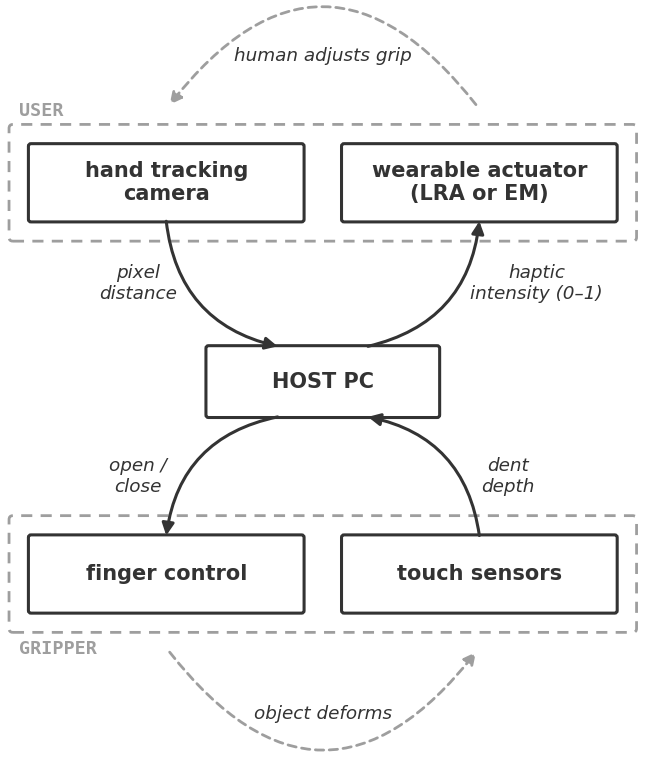
\includegraphics[width=0.85\textwidth]{preprint_fig1.png}
    \caption{Signal flow of the teleoperation loop. Everything upstream of the
        haptic driver is identical in the LRA and EM conditions; only the actuator
        and its drive stage differ.}
    \label{fig:signalflow}
\end{figure}

The loop runs at approximately \SI{30}{\hertz}, set by the tactile camera frame
rate, and is implemented as a set of cooperating threads on the host: a
tracking thread, a tactile-sensing thread, a gripper-command thread, and a
logging thread that writes one row per sensor update.

\begin{figure}[htbp]
    \centering
    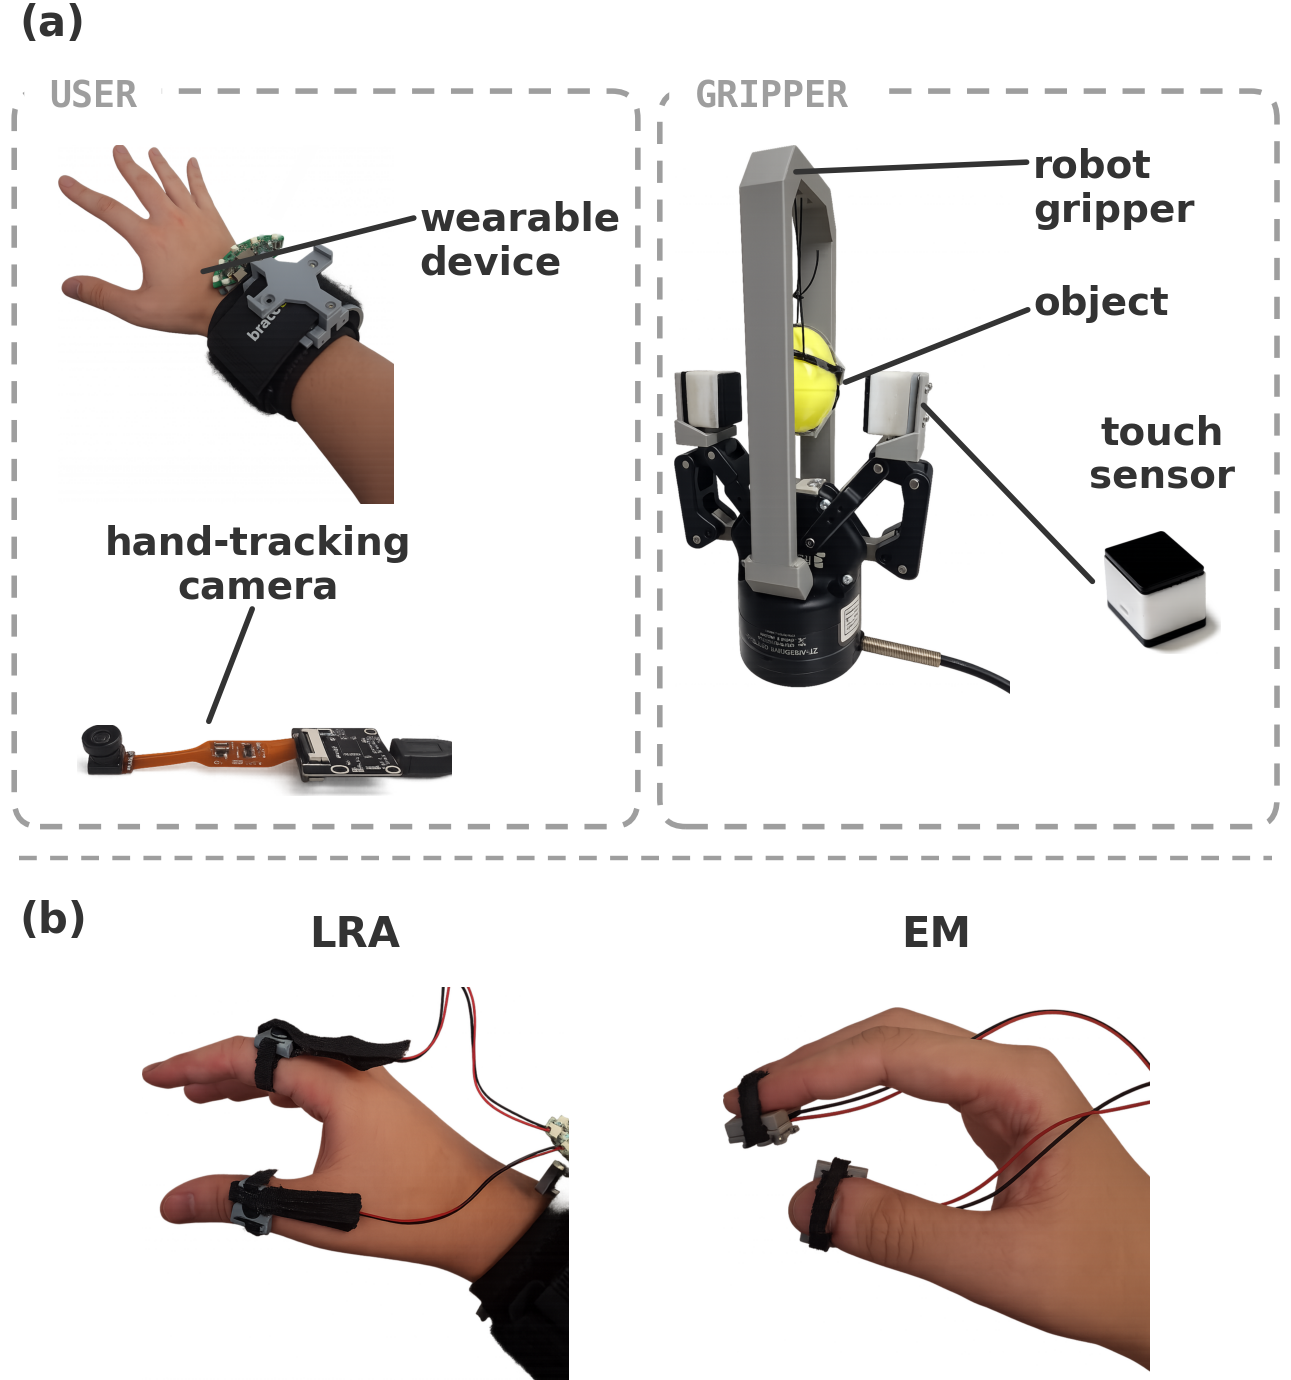
\includegraphics[width=0.9\textwidth]{preprint_fig2.png}
    \caption{Hardware. (a) The operator station and gripper apparatus, grouped
        as in Figure~\ref{fig:signalflow}. (b) The two actuator types compared in
        this study: LRA (left) and EM bistable pin (right).}
    \label{fig:hardware}
\end{figure}

\section{Operator-Side Control: Hand Tracking}
\label{sec:handtracking}

The gripper is commanded from the operator's own hand rather than from a
joystick or slider, so that the motor act of closing the gripper resembles the
motor act of closing the hand. A single RGB camera observes the operator's
dominant hand; a markerless hand-tracking model returns 2D landmark positions,
from which the thumb-tip to index-tip distance is computed each frame. This
pinch aperture is normalised against a per-participant calibration, taken from
a fully open and a fully closed pinch recorded at the start of the session, and
mapped linearly onto the gripper's commanded position register.

\todo{Add the calibration equation, the smoothing filter and its time constant,
    the dead-band used to suppress tracking jitter, and a note on the failure mode
    when the hand leaves the tracking volume.}

\section{Robotiq 2F-85 and Tactile Integration}
\label{sec:gripper}

The remote manipulator is a Robotiq 2F-85 adaptive two-finger gripper,
controlled from the host over Modbus RTU \cite{robotiq_manual}. The gripper exposes commanded
position, measured position, and motor current; the last of these is used as a
secondary, coarse indicator of grasp effort but is not the primary force proxy
in this study.

\subsection{Sensor Mounting}
\label{subsec:sensormount}

A 9DTact vision-based tactile sensor replaces the fingertip pad on the gripper
finger. The sensor comprises a deformable elastomer layer, a diffuse
illumination ring, and a camera imaging the inner surface of the layer.

\todo{Add the printed mount geometry, the standoff distance from camera to gel,
    cable routing, and a photograph of the assembled finger.}

\subsection{Calibration and Reconstruction}
\label{subsec:sensorcalib}

Calibration follows the 9DTact procedure \cite{lin2023}: a reference frame of the undeformed
gel is captured, then a ball of known radius is pressed into the gel at a set of
positions to fit the mapping from pixel intensity to indentation depth. From
this mapping, each incoming frame yields a depth map of the contact patch, from
which two quantities are derived:

\begin{itemize}
    \item \textbf{Deformation volume}: the integral of indentation depth over
          the contact patch, in arbitrary units (a.u.). This is the primary
          grip-force proxy used throughout the analysis. It is uncalibrated: it
          is monotonic in applied force but is not expressed in newtons.
    \item \textbf{Maximum indentation depth}: the peak of the depth map, in
          millimetres. This is the quantity mapped to haptic intensity.
\end{itemize}

\subsection{Depth-to-Intensity Mapping}
\label{subsec:mapping}

Maximum indentation depth $d$ is mapped to a normalised haptic intensity
$u \in [0,1]$ by clipping and linear scaling against a fixed ceiling
$d_{\max}$:
\begin{equation}
    u = \min\!\left(\frac{\max(d - d_0,\, 0)}{d_{\max} - d_0},\; 1\right),
    \label{eq:mapping}
\end{equation}
where $d_0$ is the no-contact noise floor established at calibration and
$d_{\max} = \SI{1.0}{\milli\metre}$ is a safety ceiling above which the gripper
is commanded to stop closing. Equation~\eqref{eq:mapping} is identical in both
haptic conditions; the conditions differ only in how $u$ is realised physically.

The saturation implied by Equation~\eqref{eq:mapping} has a direct experimental
consequence. Once $d$ reaches $d_{\max}$, the display stops changing, and any
further squeezing by the operator delivers no new information. Deformation
volume accumulated after that point is therefore, by construction, effort the
feedback channel could not have discouraged. This is the \emph{excess
    deformation} metric defined in Section~\ref{sec:metrics}.

\section{ESP32-C6 Haptic Driver}
\label{sec:driver}

Intensity values are streamed from the host to an ESP32-C6 over a USB serial
link as short binary packets, one per control tick. The firmware maintains the
commanded intensity for each of five channels and regenerates the corresponding
drive waveform locally, so a dropped packet degrades to a held value rather than
to silence.

\subsection{LRA Drive}
\label{subsec:lra-drive}

Each linear resonant actuator is driven differentially from an H-bridge with a
bipolar square-wave carrier at approximately \SI{200}{\hertz}. Intensity is
rendered by envelope modulation: within a fixed \SI{50}{\milli\second} window,
the carrier is gated on for a fraction of the window proportional to $u$.

This is a compromise rather than the ideal drive. An LRA's perceived amplitude
is properly modulated by varying the drive \emph{amplitude} at the actuator's
resonant frequency; the microcontroller's standard PWM peripheral cannot
generate the phase-locked antiphase pair that amplitude-modulated bipolar drive
would require. The consequence for interpretation is taken up in
Section~\ref{sec:limitations}.

\subsection{EM Bistable Pin Drive}
\label{subsec:em-drive}

Each electromagnetic actuator is a bistable pin that latches magnetically in
either the extended or retracted state and requires power only to switch between
them \cite{vechev2019}. A short H-bridge pulse of one polarity extends the pin against the
operator's fingerpad; a pulse of the opposite polarity retracts it.

Because a latched pin produces no ongoing sensation, a sustained, graded
percept is approximated by repeated pulsing: intensity $u$ is mapped to the
burst-to-gap ratio of an extend/retract pulse train, so that higher intensity
produces more frequent contact events per unit time.

\todo{Insert the schematic of the five-channel driver board, the H-bridge part
    number, supply voltage and current budget, and the measured pulse width required
    for reliable latching.}

\section{Data Logging}
\label{sec:logging-arch}

The host writes one CSV row per control tick for the duration of each recorded
trial, containing the timestamp, commanded and measured gripper position, motor
current, deformation volume, maximum indentation depth, the rendered haptic
intensity, and the active control mode. These logs are the sole source of the
quantitative metrics in Chapter~\ref{ch:results}.

% =====================================================================
\chapter{Experimental Methodology}
\label{ch:methodology}
% =====================================================================

\section{Participants}
\label{sec:participants}

Twenty-two participants ($N=22$) took part in the study. Eligibility required
normal or corrected-to-normal vision and no diagnosed sensory or motor
impairment affecting the dominant hand; a screening item recorded any such
impairment and was used to exclude affected responses from the subjective
analysis. Prior robotics or teleoperation experience was not required, and was
recorded as a covariate. All participants gave informed consent before taking
part.

The sample exceeds the $N=10$--$12$ typical of comparable vibrotactile
teleoperation studies, which was the target set during design; the larger sample
was recruited to improve power for the actuator-versus-actuator comparison,
which was expected a priori to have a smaller effect than the
feedback-versus-no-feedback comparison.

\section{Design and Counterbalancing}
\label{sec:design}

The study uses a within-subjects design with one factor, feedback condition, at
three levels: \textbf{visual-only} (V), \textbf{LRA}, and \textbf{EM}. Every
participant experienced all three conditions, which controls for individual
differences in manual dexterity and grip-force perception that would otherwise
dominate a between-subjects comparison at this sample size.

\todo{State the realised condition order explicitly. The presentation preprint
    records the order as fixed rather than counterbalanced; if that is correct, this
    section must say so plainly here and the resulting practice/fatigue confound
    must be carried into Section~\ref{sec:limitations} rather than described as
    controlled.}

Within each condition, participants performed five trials per object class,
giving ten trials per condition and thirty trials per participant, and 110
trials per condition per object class across the sample.

\section{Task and Materials}
\label{sec:task}

Participants sat at a workstation facing a display carrying the remote-view
camera feed, with no direct line of sight to the gripper. In the LRA and EM
conditions they wore the corresponding actuator array on the fingertips of the
dominant hand. The gripper stood vertically with its fingers pointing upward;
each object was presented in a fixed cradle at the end of a horizontal support
arm, positioned so that the object centre sat at a constant height of
\SI{16.5}{\centi\metre} aligned with the centre of the open finger gap. The
gripper body did not move during a trial: only the fingers opened and closed,
under hand-tracking control.

Each trial consisted of closing the gripper on the presented object, holding
briefly, and releasing it without dropping or visibly damaging it. Two object
classes were used, shown in Figure~\ref{fig:objects}:

\begin{itemize}
    \item \textbf{Fragile}: a hollow two-part plastic egg, which separates
          abruptly once the applied force exceeds the seam strength. Failure is
          discrete and unambiguous, and the object is replaced between trials.
    \item \textbf{Deformable}: a foam cube, which yields progressively and
          recovers between trials, with no discrete failure point.
\end{itemize}

\begin{figure}[htbp]
    \centering
    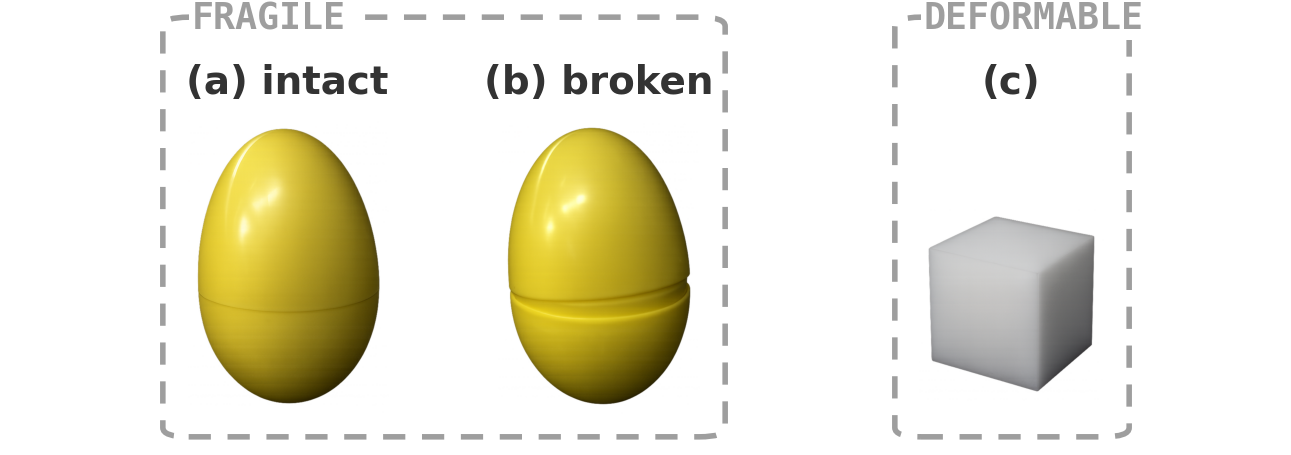
\includegraphics[width=0.85\textwidth]{preprint_fig4.png}
    \caption{Object classes. (a) The hollow plastic egg used as the fragile
        object. (b) The same egg with its halves separated, the failure event scored
        as breakage. (c) The foam cube used as the deformable object.}
    \label{fig:objects}
\end{figure}

\section{Session Protocol}
\label{sec:protocol}

Figure~\ref{fig:methodflow} summarises the session. Each session comprised:
(1) informed consent and task explanation; (2) per-participant pinch
calibration; (3) an untimed practice trial in each condition, in the order the
participant would encounter them, with no data recorded; (4) the three
experimental conditions, each completed in full before moving to the next;
(5) a post-condition questionnaire administered immediately after each
condition; and (6) a closing preference question and free-form interview.
Rest breaks were offered between conditions.

\begin{figure}[htbp]
    \centering
    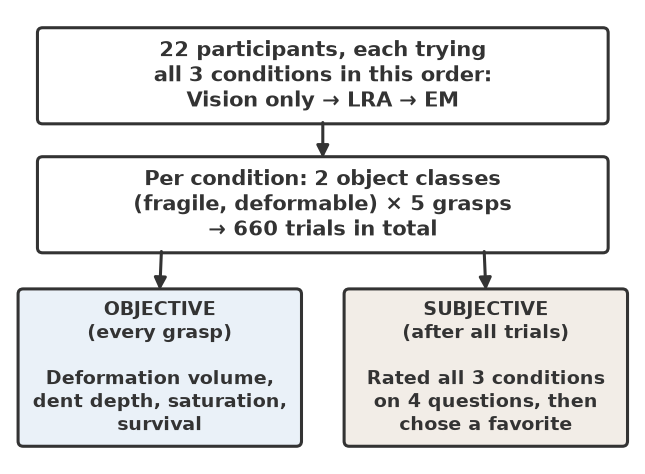
\includegraphics[width=0.8\textwidth]{preprint_fig3.png}
    \caption{Flowchart of the experimental session, $N=22$.}
    \label{fig:methodflow}
\end{figure}

\section{Instruments}
\label{sec:instruments}

\subsection{Quantitative Logging}
\label{subsec:logging}

Per-tick logs are as described in Section~\ref{sec:logging-arch}. Object
outcome, survived or broke, for fragile objects, was scored by the
experimenter immediately after each trial and recorded alongside the log.

\subsection{Post-Condition Questionnaire}
\label{subsec:questionnaire}

After each condition, participants rated a set of 7-point Likert items
(1 = strongly disagree, 7 = strongly agree) covering perceived force awareness,
contact detection, damage anticipation, mental effort, and sense of control.
Two further items, administered only in the LRA and EM conditions, addressed the
perceived responsiveness and naturalness of the feedback itself. A single
forced-choice preference question at the end of the session asked which
condition the participant would choose to perform the task again.

\todo{Reproduce the exact item wording as administered, in
    Appendix~\ref{app:questionnaire}, and confirm the item numbering used by the
    analysis pipeline matches it.}

\section{Analysis Procedures}
\label{sec:analysis-procedures}

Per-trial metrics (Section~\ref{sec:metrics}) are reduced to one value per
participant per condition per object class using the median across repeated
trials, so that a single unusually careless grasp cannot dominate a
participant's contribution. Cross-condition comparisons use the Friedman test,
the non-parametric repeated-measures analogue of one-way ANOVA, with pairwise
Wilcoxon signed-rank tests and Holm correction across the three condition pairs
where the omnibus test is significant. Fragile-object survival, being a paired
binary outcome, is tested with McNemar's test. Results are reported as medians
and interquartile ranges rather than means and standard deviations, for
robustness to the high-force outliers the study is designed to detect. All
analyses are implemented in the accompanying \texttt{analysis} package and
regenerate the tables and figures of Chapter~\ref{ch:results} from the raw logs.
CSV outputs referenced by filename in Chapter~\ref{ch:results} are written to
\texttt{analysis/results/}.

% =====================================================================
\chapter{Results}
\label{ch:results}
% =====================================================================

\section{Derived Per-Trial Metrics}
\label{sec:metrics}

Four metrics are computed from each trial log:

\begin{itemize}
    \item \textbf{Peak deformation volume} (a.u.): the maximum deformation
          volume reached during the trial; the primary grip-force proxy.
    \item \textbf{Excess deformation} (a.u.): deformation volume accumulated
          after maximum indentation depth has plateaued, i.e.\ after the haptic
          display has saturated per Equation~\eqref{eq:mapping} and further
          squeezing conveys nothing new.
    \item \textbf{Grip adjustments} (count): the number of squeeze/release
          reversals after the plateau, taken as a sign of searching for an
          appropriate grip rather than holding steady.
    \item \textbf{Peak indentation depth} (\si{\milli\metre}): the maximum of
          the depth map, reported mainly as a check on the safety ceiling.
\end{itemize}

\section{Fragile Objects}
\label{sec:results-fragile}

Table~\ref{tab:quant} summarises the fragile-object results.

\begin{table}[htbp]
    \centering
    \caption{Fragile-object results by condition (V = visual only). The first
        four rows give the median value for a participant, where lower is better.
        The last row is the percentage of all 110 trials per condition in which the
        object survived. Peak indentation depth differs little across conditions
        because the \SI{1.0}{\milli\metre} safety ceiling caps it before any
        difference could emerge.}
    \label{tab:quant}
    \begin{tabular}{@{}lrrr@{}}
        \toprule
                                       & V     & LRA   & EM    \\
        \midrule
        Peak deformation volume (a.u.) & 20100 & 12300 & 16000 \\
        Excess deformation (a.u.)      & 1530  & 170   & 260   \\
        Grip adjustments (\#)          & 7     & 5     & 2     \\
        Peak indentation depth (mm)    & 0.98  & 0.95  & 0.98  \\
        \midrule
        Objects surviving (\%)         & 62    & 81    & 78    \\
        \bottomrule
    \end{tabular}
\end{table}

Both haptic conditions reduced the force applied after the display had
saturated: median excess deformation fell roughly ninefold under the LRA and
roughly sixfold under the EM relative to visual-only feedback. Grip adjustments
fell most under the EM condition. Object survival rose from 62\% under
visual-only feedback to 81\% (LRA) and 78\% (EM), as shown in
Figure~\ref{fig:results}.

\begin{figure}[htbp]
    \centering
    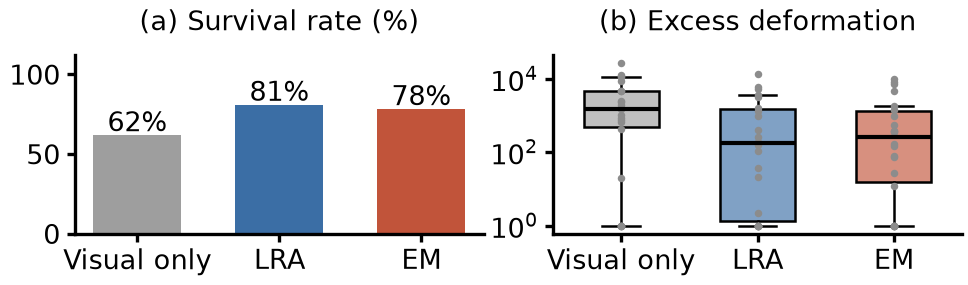
\includegraphics[width=0.9\textwidth]{preprint_fig5.png}
    \caption{Objective results for fragile objects. (a) Survival rate, 110
        trials per condition. (b) Excess deformation per participant (a.u.,
        $\log(x+1)$ scale).}
    \label{fig:results}
\end{figure}

\todo{Insert the omnibus Friedman statistics, the Holm-corrected pairwise
    $p$-values, and the McNemar result for survival, from the analysis outputs
    \texttt{section\_5\_3\_cross\_condition.csv} and
    \texttt{section\_5\_4\_fragile\_mcnemar.csv}. Report effect sizes alongside
    $p$-values.}

\section{Deformable Objects}
\label{sec:results-deformable}

Deformable objects showed no reliable difference between conditions on any of
the four metrics. This is consistent with the nature of the object class: a foam
cube has no failure threshold to avoid, so there is no penalty for squeezing
harder and correspondingly little for the feedback channel to correct.

\todo{Report the deformable-object table in the same format as
    Table~\ref{tab:quant}, together with the omnibus tests, so that the null result
    is stated with statistics rather than asserted.}

\section{Sensor-to-Actuator Latency}
\label{sec:latency}

\todo{Outstanding. The trial logs are timestamped at the control-loop rate
    ($\approx$\SI{30}{\hertz}) but do not establish true end-to-end latency from
    tactile frame capture to physical actuator motion. A bench measurement is
    required, combining a frame-capture timestamp, a serial packet timestamp, and
    either an oscilloscope or photodiode trigger on the actuator itself, reported
    once per
    actuator type as a latency distribution.}

\section{LRA Versus EM}
\label{sec:lra-vs-em}

Because the two haptic conditions share an identical sensing and
intensity-computation pipeline, a direct paired comparison between them isolates
the actuator-type variable. On the fragile-object metrics the two conditions
are close: the LRA yields the lower median excess deformation and the EM the
lower number of grip adjustments, and neither difference is large relative to
the spread across participants.

\todo{Insert the paired Wilcoxon results from
    \texttt{section\_5\_4\_lra\_vs\_em.csv} and the equivalence
    test from \texttt{section\_5\_9\_tost\_equivalence.csv}. If the TOST result
    supports equivalence within the chosen bound, say so explicitly: a null result
    and a demonstrated equivalence are different claims and should not be
    conflated.}

\section{Time-Series Behaviour}
\label{sec:timeseries}

Representative single-trial traces for each condition illustrate the behaviour
the excess-deformation metric is designed to capture: under visual-only
feedback, deformation volume continues to rise after indentation depth has
plateaued, whereas under both haptic conditions it tends to level off shortly
after the plateau.

\begin{figure}[htbp]
    \centering
    \begin{subfigure}[b]{0.48\textwidth}
        \centering
        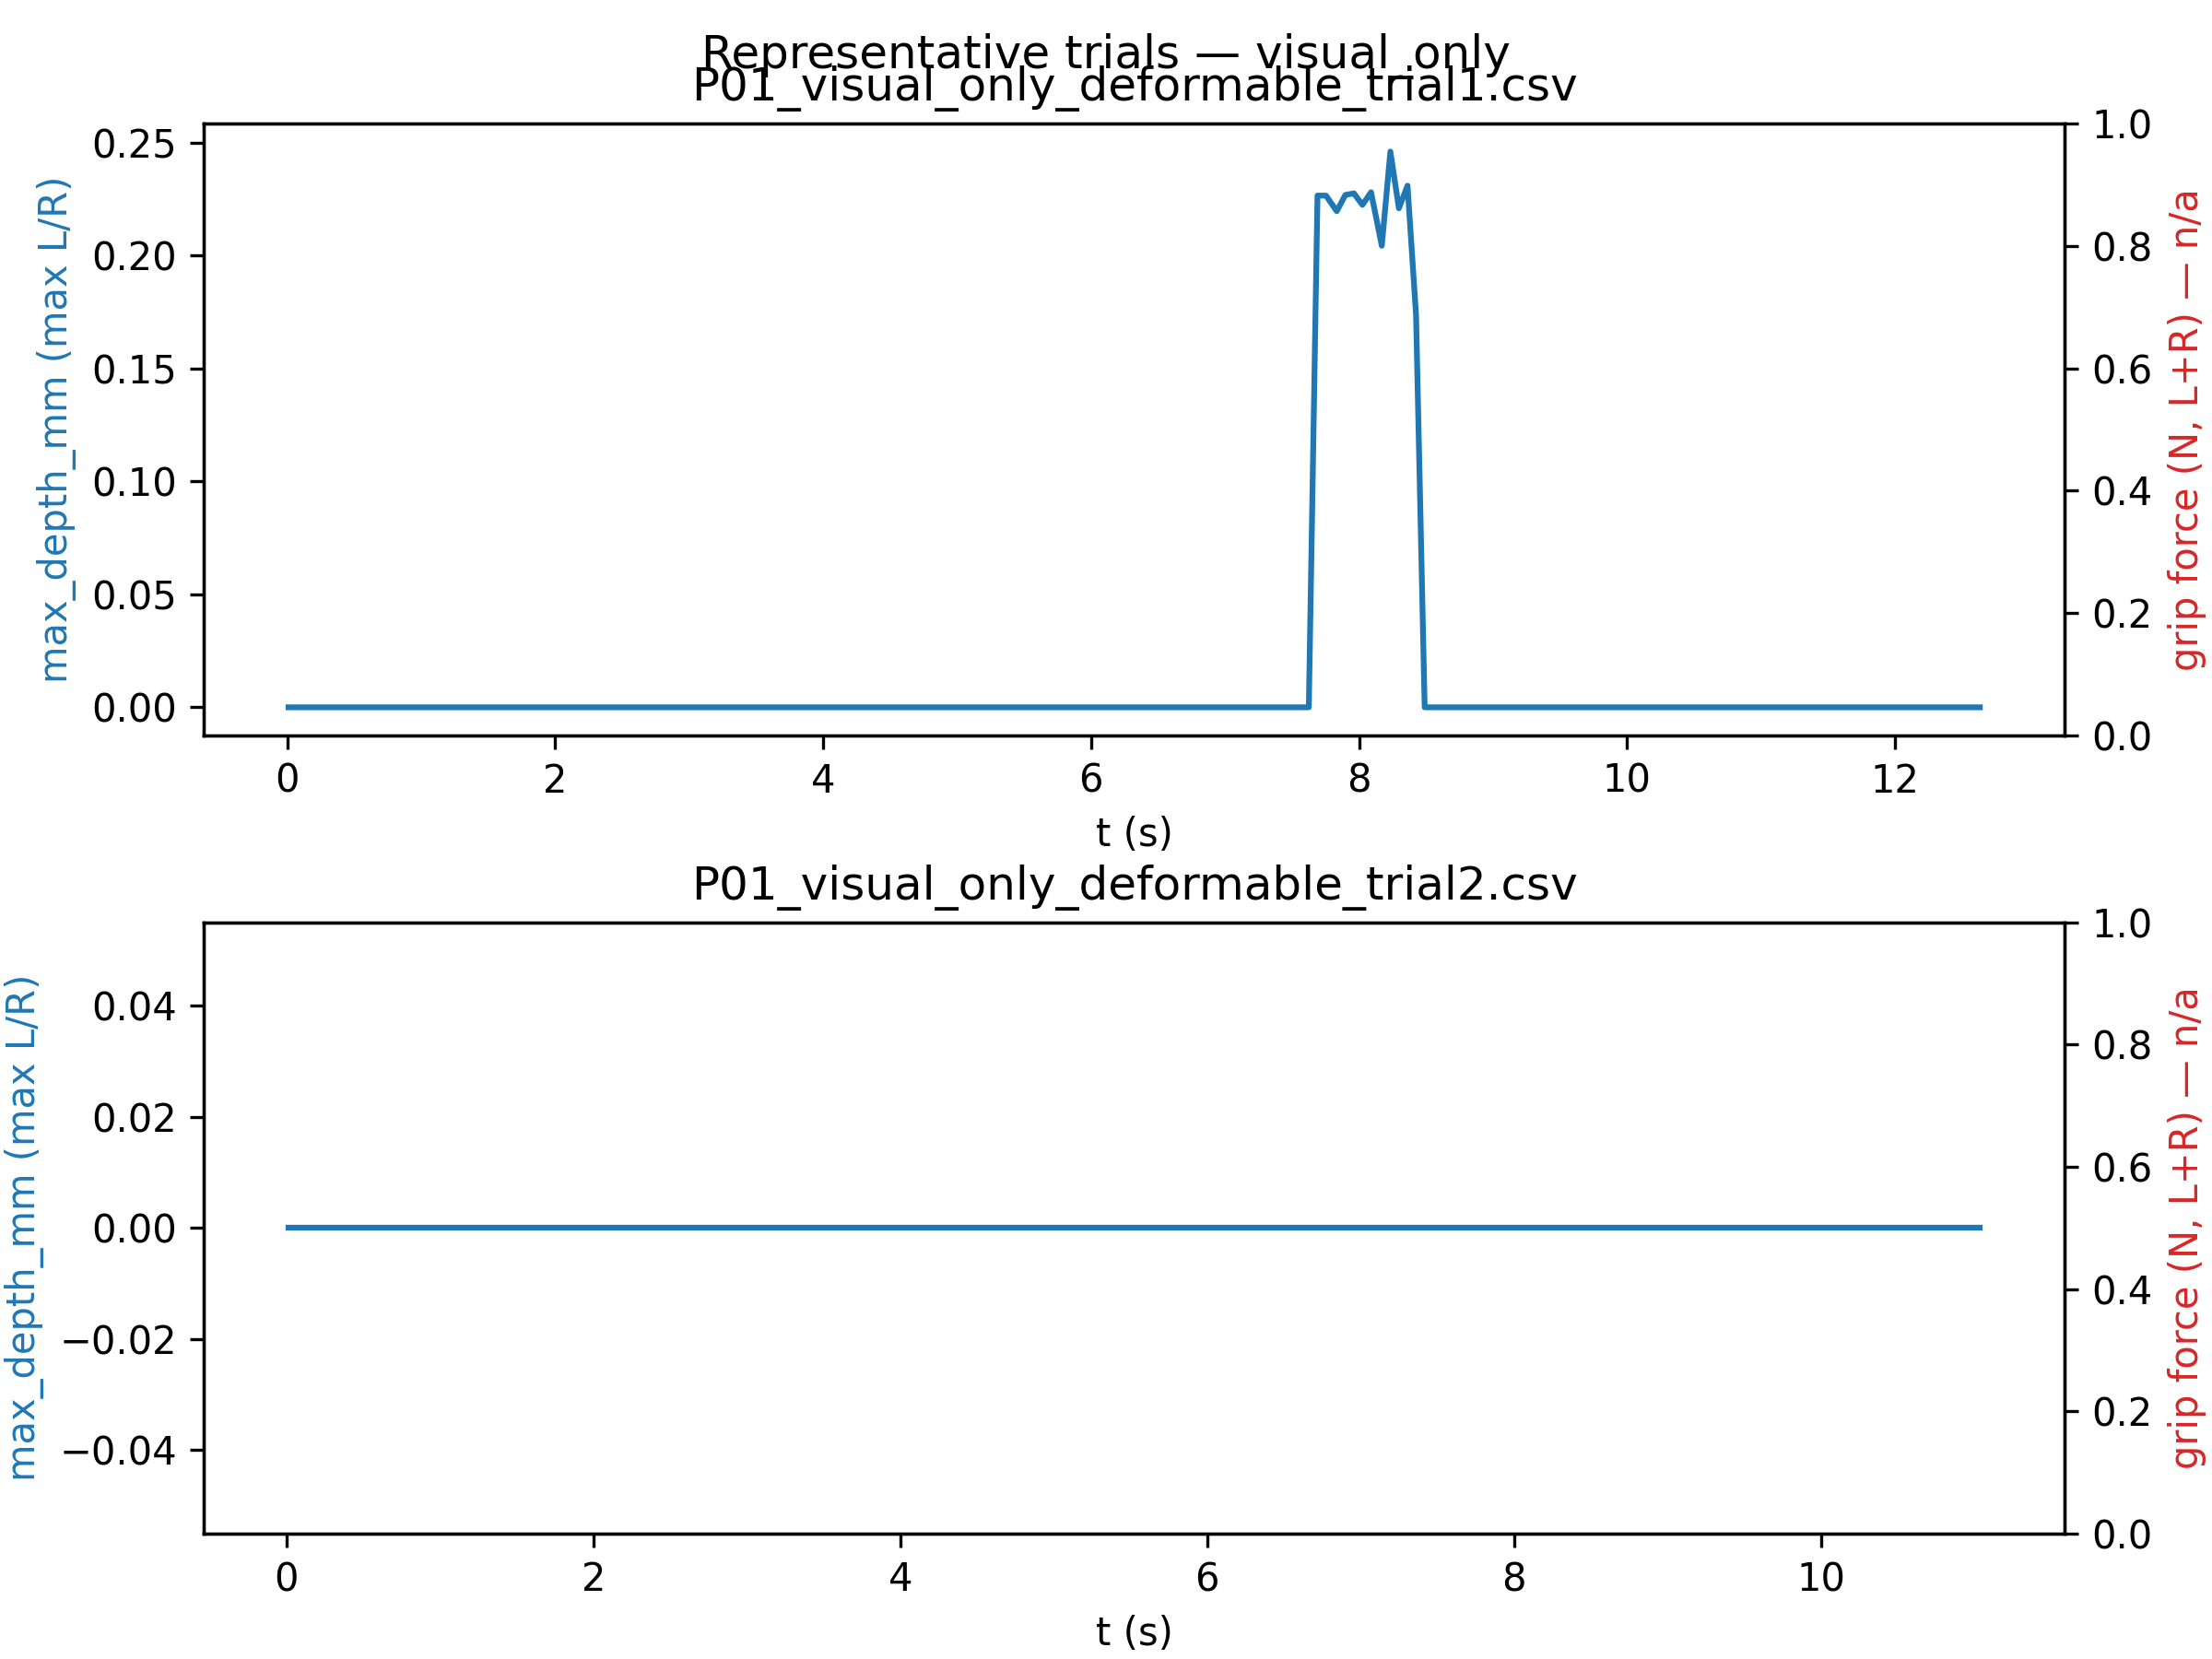
\includegraphics[width=\textwidth]{section_5_5_timeseries_visual_only.png}
        \caption{Visual-only}
    \end{subfigure}
    \hfill
    \begin{subfigure}[b]{0.48\textwidth}
        \centering
        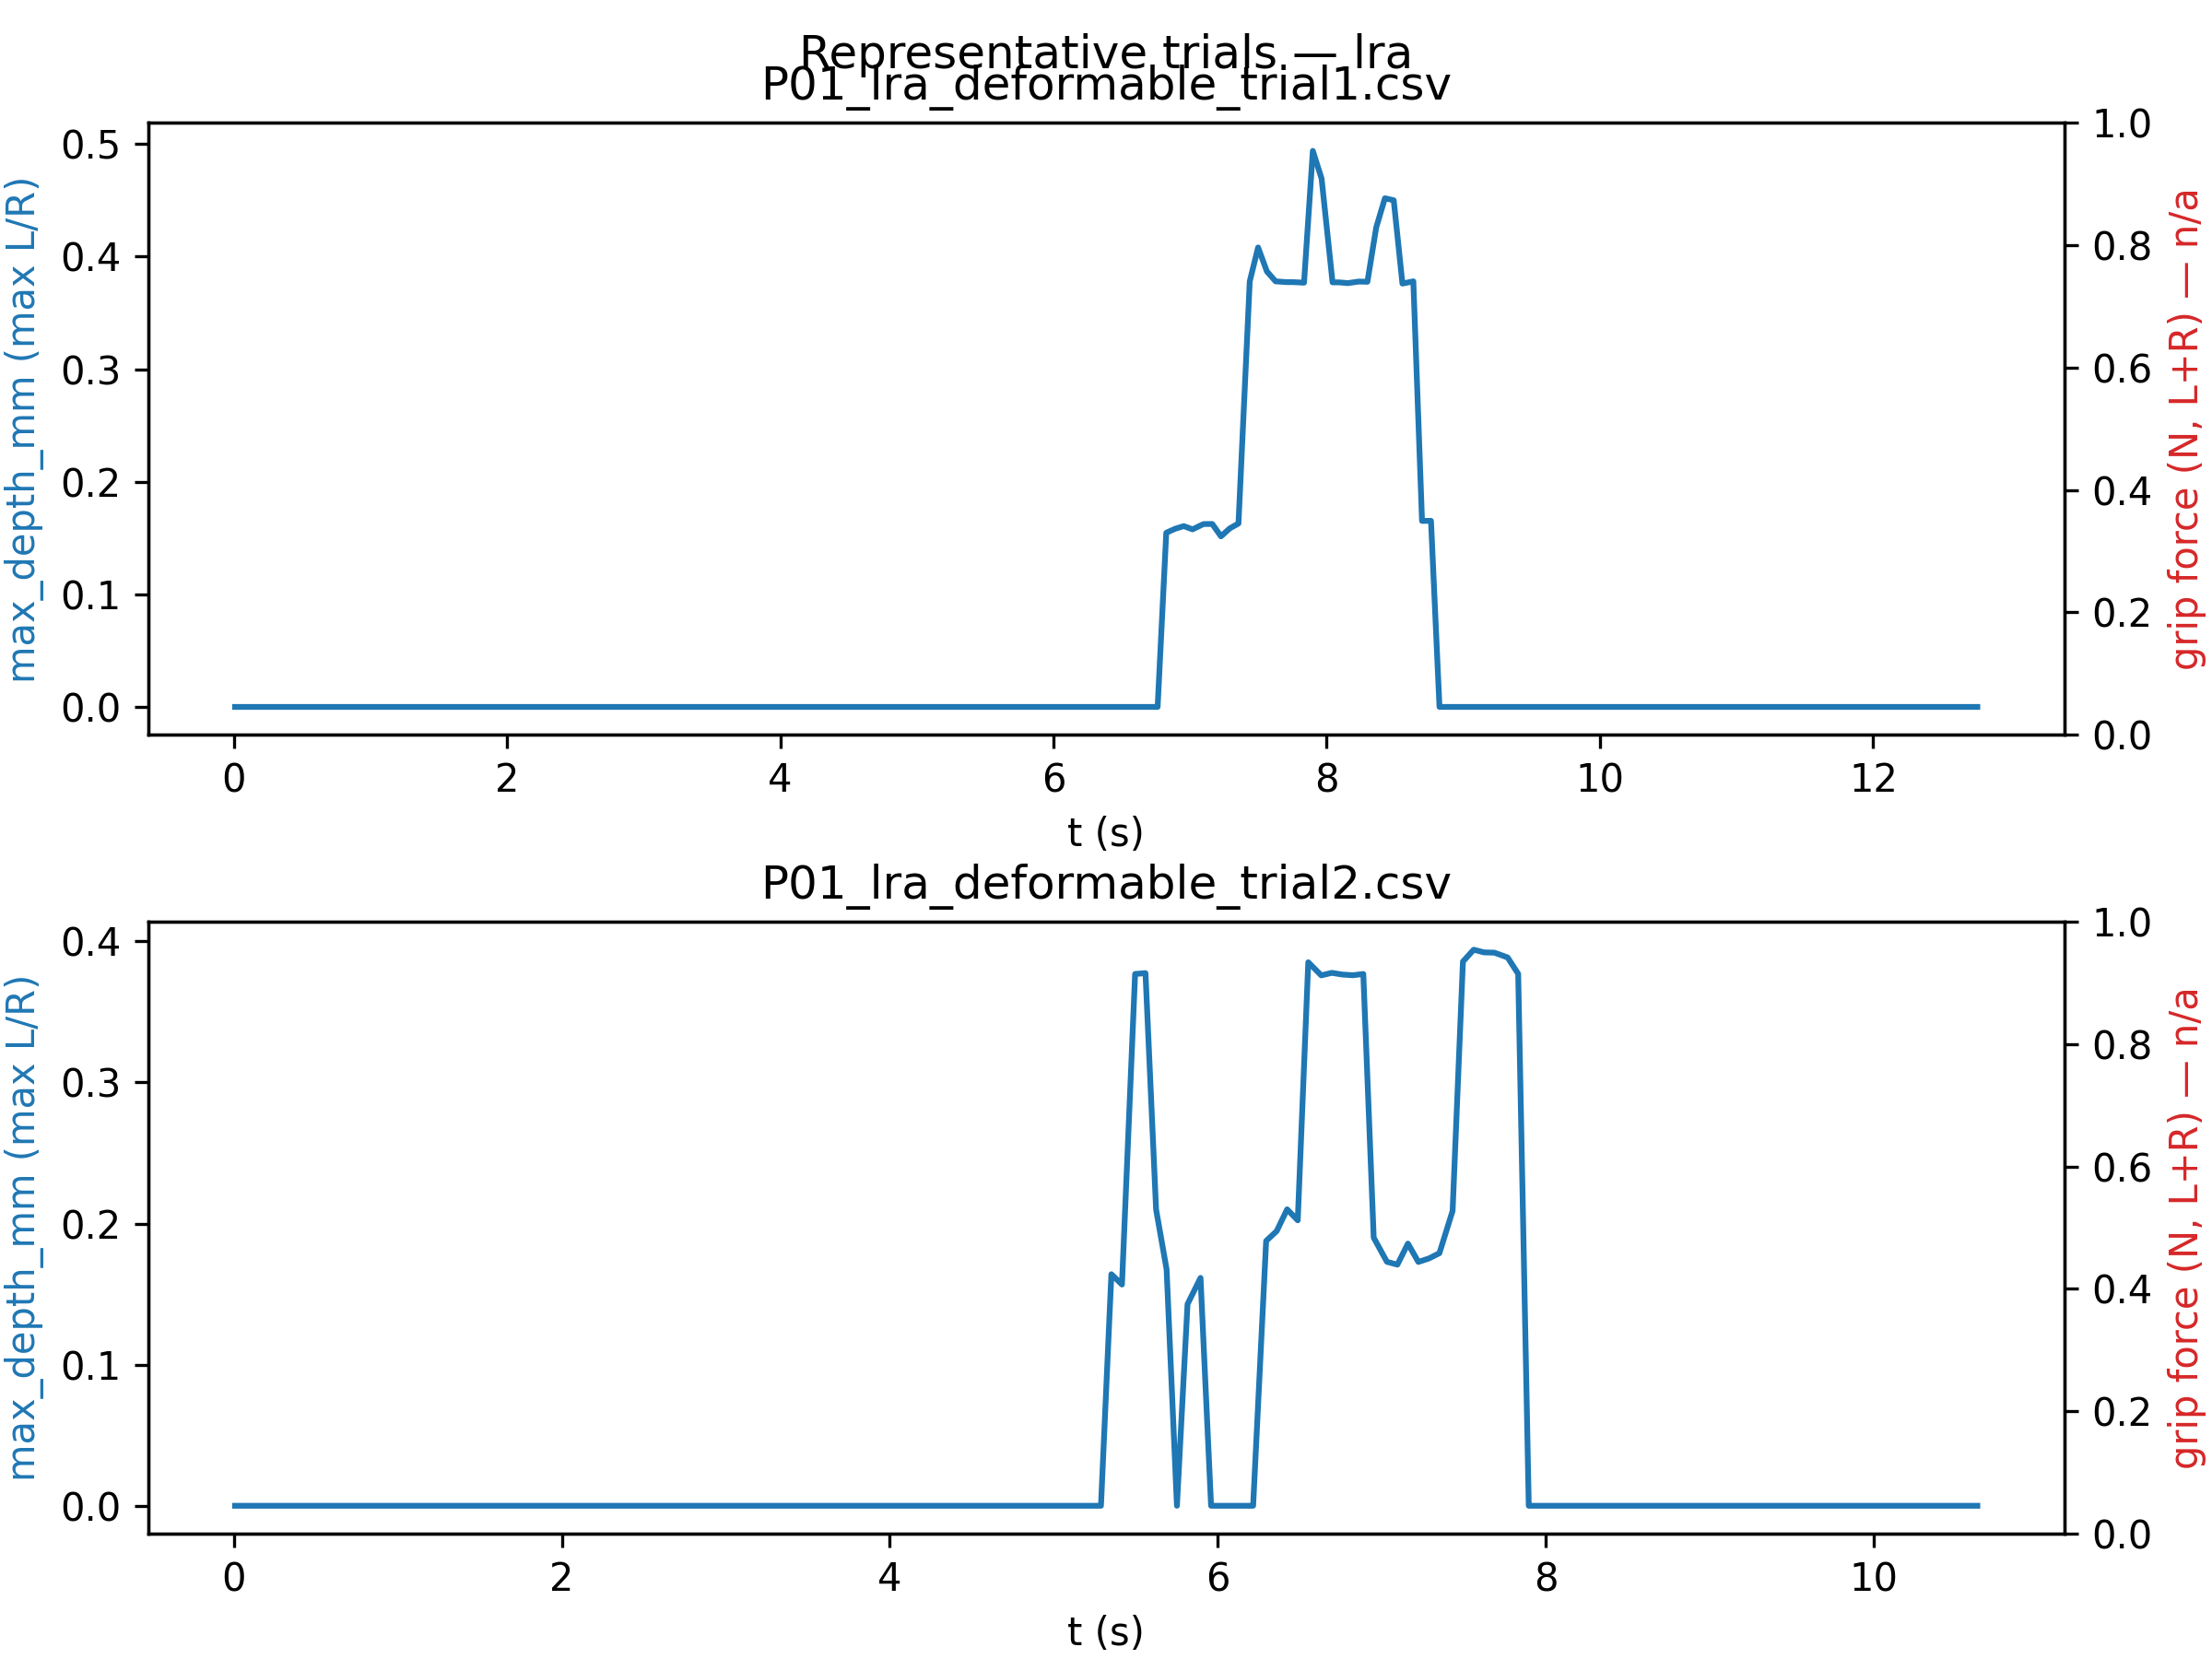
\includegraphics[width=\textwidth]{section_5_5_timeseries_lra.png}
        \caption{LRA}
    \end{subfigure}
    \\[1ex]
    \begin{subfigure}[b]{0.48\textwidth}
        \centering
        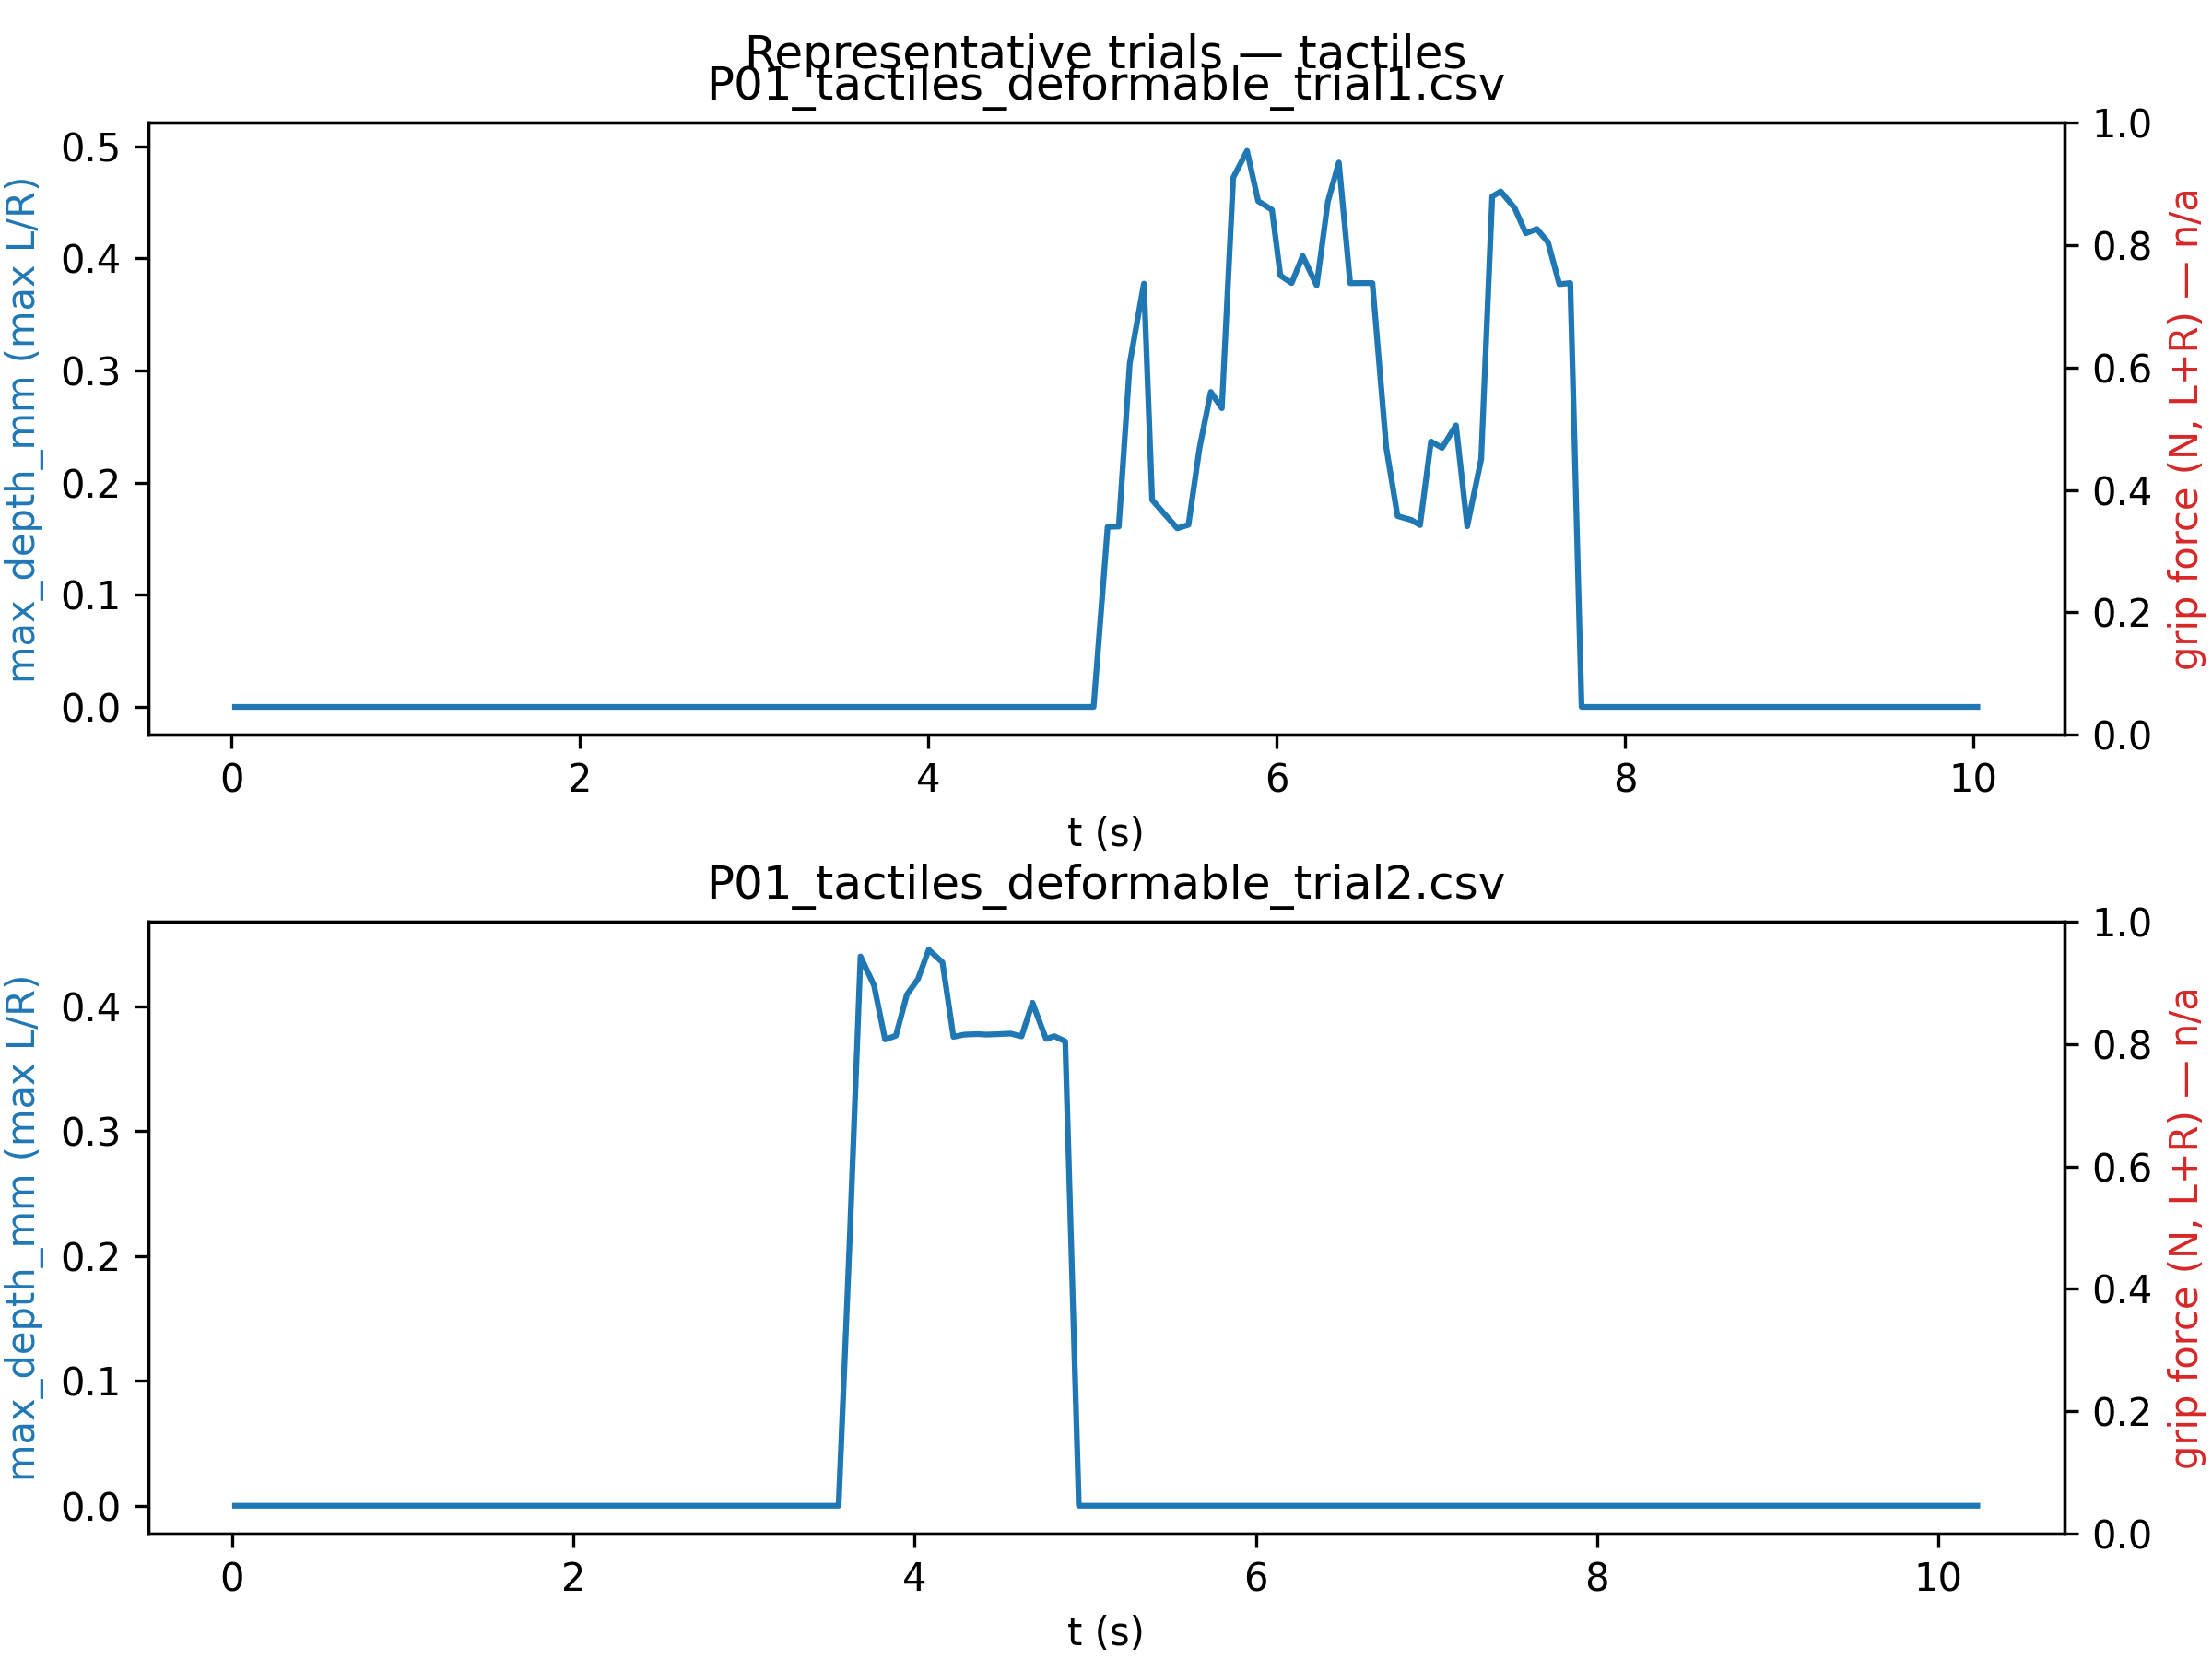
\includegraphics[width=\textwidth]{section_5_5_timeseries_em.png}
        \caption{EM}
    \end{subfigure}
    \caption{Representative single-trial traces of indentation depth and
        deformation volume against time, one per feedback condition.}
    \label{fig:timeseries}
\end{figure}

\section{Subjective Results}
\label{sec:results-likert}

Participants rated both haptic conditions above visual-only feedback, most
strongly on items concerning the ability to feel grip force and confidence in
the grasp (Figure~\ref{fig:likert}). In the forced-choice preference question
the LRA was the most frequently selected condition. No individual questionnaire
item separated the two haptic conditions reliably.

\begin{figure}[htbp]
    \centering
    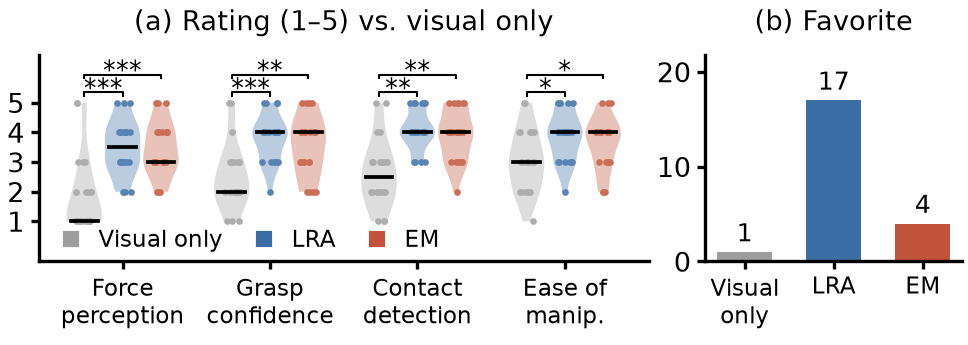
\includegraphics[width=0.9\textwidth]{preprint_fig6.png}
    \caption{Subjective results. (a) Item-by-item ratings relative to
        visual-only feedback, $N=22$; additional star marks indicate stronger
        statistical reliability. (b) Share of forced-choice favourite picks per
        condition.}
    \label{fig:likert}
\end{figure}

\todo{Insert the per-item medians and IQRs and the Friedman/Wilcoxon statistics
    from \texttt{section\_5\_6\_likert\_summary.csv} and
    \texttt{section\_5\_6\_likert\_friedman.csv}, and the preference counts from
    \texttt{section\_5\_6\_likert\_preference.csv}.}

% =====================================================================
\chapter{Discussion}
\label{ch:discussion}
% =====================================================================

\section{Interpretation}
\label{sec:interpretation}

The results separate cleanly into a strong effect and a weak one.

The strong effect is the presence of tactile feedback. For fragile objects, both
haptic conditions reduced excess deformation by roughly an order of magnitude
and raised survival by 16--19 percentage points over visual-only feedback. The
mechanism is visible in the time-series traces: under visual-only feedback the
operator has no signal that indicates when the useful part of the grasp is
complete, and continues to squeeze after contact is fully established. The
haptic conditions supply exactly that signal, and the metric most improved is
the one that measures effort applied after the signal saturates. That the effect
appears in survival, not merely in the force proxy, is what makes it
practically meaningful.

The weak effect is actuator type. The LRA produced the lower excess deformation
and was the more frequently preferred condition; the EM produced fewer grip
adjustments. Neither difference is large relative to between-participant spread,
and no questionnaire item distinguished the two. The honest reading is that this
study establishes that feedback helps, and does not establish which actuator
helps more.

The absence of any effect on deformable objects is not a failure of the system
but a property of the task. A foam cube imposes no penalty for over-squeezing,
so a channel whose value lies in discouraging over-squeezing has nothing to act
on. This asymmetry is itself informative: it suggests the benefit of tactile
feedback in teleoperation is concentrated in tasks with a failure threshold
rather than distributed across manipulation generally.

\section{Limitations}
\label{sec:limitations}

Several features of the study bound how strongly these conclusions can be
stated.

\paragraph{Condition order.} Conditions were presented in a fixed order rather
than counterbalanced across participants. Practice effects across the session
and fatigue toward its end are therefore confounded with condition, and a
difference attributed to an actuator may in part reflect its position in the
session.

\paragraph{The two actuators differ in more than one way.} They differ in
transduction mechanism, but also in placement on the hand and in how well hand
tracking performed while each was worn. A preference for one actuator may
therefore reflect smoother control rather than a better sensation.

\paragraph{Rendering narrows the intended contrast.} The intended contrast was
continuous versus discretely-switched rendering. In practice the LRA is driven
by envelope modulation of a fixed-amplitude carrier rather than by true
amplitude modulation (Section~\ref{subsec:lra-drive}), so both conditions set
intensity by gating a waveform on and off, differing chiefly in temporal
granularity. A dedicated resonant-driver IC capable of amplitude modulation
would sharpen the contrast.

\paragraph{Off-resonance carrier.} The LRA carrier was set empirically to
approximately \SI{200}{\hertz} rather than tuned to the measured resonance of
the specific actuators. Since an LRA is efficient only in a narrow band around
resonance, the achievable amplitude range, and therefore the perceptual dynamic
range of the intensity signal, may have been compressed.

\paragraph{Differing native temporal response.} The LRA requires several drive
cycles to ring up and ring down; the EM latch transitions almost instantly. A
comparison intended to isolate rendering style is therefore partly a comparison
of responsiveness.

\paragraph{Uncalibrated force.} Grip force is inferred from deformation volume
in arbitrary units, not measured in newtons, and indentation depth rests on a
single-ball calibration never checked against an independent gauge, so its
millimetre scale carries unquantified error.

\paragraph{Tracking and latency.} Hand tracking is 2D and uncalibrated, and the
end-to-end sensor-to-actuator latency still requires the bench measurement
described in Section~\ref{sec:latency}.

\section{Energy-Based Modelling of the Loop}
\label{sec:phs}

At an abstract level the system is an interconnection of energy-exchanging
subsystems, namely the gripper-object contact, the sensing and computation
pipeline, and the actuator-skin interface. Teleoperation is commonly analysed
this way, treating each subsystem as a two-port element and using passivity of
the resulting energy flow as a sufficient condition for stability, an approach
that extends to port-based models of the whole loop \cite{niemeyer2016}. A full
port-Hamiltonian treatment of this system, with the contact, the tactile
sensor's deformation measurement, and the EM actuator's stored magnetic energy
each modelled as a port, lies beyond the scope of this thesis, but would
offer a principled account of why one actuator class transmits sensed
deformation more transparently than another, grounded in the energetics of the
loop rather than in empirical comparison alone.

% =====================================================================
\chapter{Conclusion}
\label{ch:conclusion}
% =====================================================================

This thesis presented an end-to-end tactile-haptic teleoperation system that
integrates vision-based tactile sensing into a Robotiq 2F-85 adaptive gripper,
commands the gripper from the operator's own pinch aperture, and renders the
sensed contact deformation on a five-channel wearable actuator array through
either linear resonant actuators or electromagnetic bistable pin actuators,
with an identical sensing and intensity-mapping pipeline upstream of the driver
in both cases.

A within-subjects study with $N=22$ participants found that tactile feedback
made the grasping of fragile objects substantially safer: excess deformation
(force applied after the tactile display had saturated) fell by close to
an order of magnitude, and object survival rose from 62\% under visual-only
feedback to 81\% with the LRA and 78\% with the EM. Deformable objects, which
lack a failure threshold, showed no reliable effect. Participants preferred both
haptic conditions to visual-only feedback and most often chose the LRA, but no
questionnaire item separated the two actuators reliably.

The conclusion is therefore asymmetric, and deliberately so: the presence of
tactile feedback matters, and the choice between these two actuators, under
these conditions and at this sample size, does not demonstrably matter. Ranking
actuator types would require a study that removes the confounds identified in
Section~\ref{sec:limitations}: counterbalanced condition order, matched
placement on the hand, resonance-tuned amplitude-modulated LRA drive, and a
force proxy calibrated in newtons.

Future work follows directly from these limitations, and from one extension the
present system does not exploit: the tactile sensor produces a full depth map,
of which this study renders a single scalar per finger. Rendering the spatial
structure of the contact patch across the actuator array, rather than
collapsing it to one intensity, is the most promising direction for
recovering more of the information the sensor already measures.

% =====================================================================
%  BACK MATTER
% =====================================================================
\cleardoublepage
\begingroup
\raggedright
\printbibliography[heading=bibintoc, title={References}]
\endgroup

\appendix
\cleardoublepage

\chapter{Questionnaire Items}
\label{app:questionnaire}
\todo{Reproduce the questionnaire exactly as administered, including the
    demographic and screening items and the closing preference question.}

\chapter{Per-Participant Summary Data}
\label{app:data}
\todo{Table of per-participant, per-condition medians for each metric of
    Section~\ref{sec:metrics}, generated from
    \texttt{section\_5\_1\_reduced\_metrics.csv}.}

\chapter{Firmware and Driver Details}
\label{app:firmware}
\todo{Driver schematic, bill of materials, pulse-timing parameters, and the
    serial packet format used between host and ESP32-C6.}

\cleardoublepage
\chapter*{Acknowledgements}
\addcontentsline{toc}{chapter}{Acknowledgements}
\todo{Acknowledge \supervisorname, the laboratory, and the study participants.}

\end{document}
